\section{Approach}\label{s:approach}


Creating a categorical split between LC and BE in the scheduler solves these
problems, and the infrastructure for doing so already exists in Linux.

\subsection{A better interface: categorical separation}\label{ss:interface}

A categorical differentiation in the scheduler enables unbounded unfairness
towards BE during high load, and requires few and well-defined synchronization
points between cores.

Unbounded unfairness is a requirement for practical independence between LC and
BE workloads: LC service times need to be independent of the load as well as the
number of BE workloads. For any weighted split, a large enough number of BE
workloads will add up to a significant weight in the system; for example, even
if the weights were correctly globally enforced, packing 100 BE workloads on a
machine would lead the proportional weight of the LC workload to decrease
significantly. A categorical split between LC and BE avoids this: as more BE
workloads start up, the share that BE gets doesn't change. As a resultof this
unbounded unfairness towards BE workloads, we have bounded the amount of impact
that BE workloads can have on LC workloads' CPU time.

Creating separate categories also allows for fewer synchronization points
without losing any of the global guarantees. In order to enforce a categorical
priority, the scheduler only needs to sychronize at two points: on
\textit{entry}, when a new high-priority thread wakes up on a core already
running something high-priority, and \textit{exit}, when starting to run a low
priority thread. If on entry the scheduler looks for cores running low priority
work to go interrupt, and on exit the scheduler looks for high priority work to
steal, it has ensured the global property that \textit{no core is ever running a
BE process while an LC one is runnable and waiting}.


\subsection{Linux already does it}

There is a way to configure tasks so that Linux enforces global priorities:
processes that run in real time have strict priority over other processes.

Each scheduling class exists completely separately: classes maintain their own
run queues and per-entity state; implement their own scheduling algorithms to
choose from the entities on their runqueue; and balance the load across
runqueues on different cores.

Linux isolates strictly between different scheduling classes: it only schedules
a lower scheduling class if the higher scheduling classes found nothing to run,
and each scheduling class tries to steal work from other cores before returning
that it has nothing to run --- these two checks represent the entry and exit
synchronization points. It is thereby true that if something in the Normal
scheduling class is running, it means there are no Fifo tasks waiting to run
anywhere on the machine.

This points to a possible solution: run LC in the Fifo scheduling class and BE
in Normal.\footnote{The Deadline scheduling class is not a good fit, since it
requires accurate knowledge of a processes runtime (processing time per request)
and period (when requests come in)} Fifo runs a priority scheduler: it has 99
priorities, each takes strict precedent over the one lower; within priorities
the scheduler enforces a global first-in-first-out (hence the Fifo class name),
based on when processes become runnable.

\begin{figure}[t]
    \centering
    \begin{subfigure}[t]{0.48\columnwidth}
        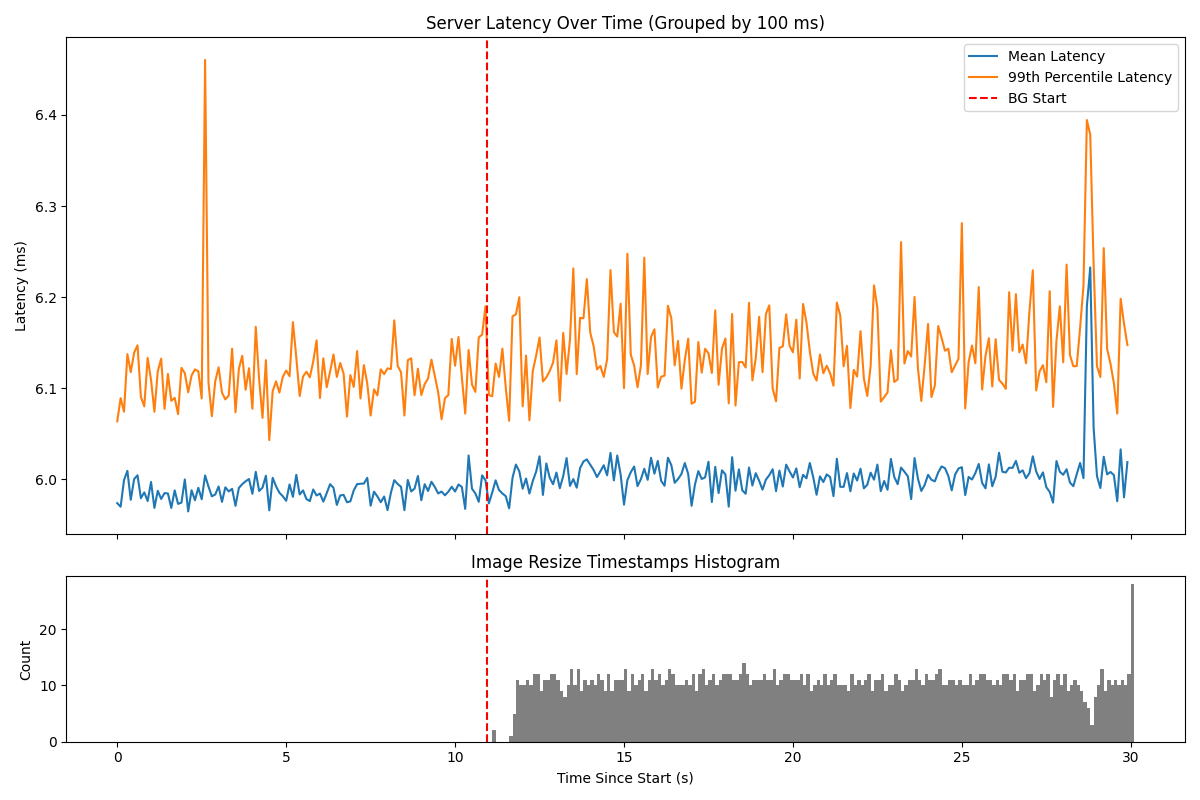
\includegraphics[width=\columnwidth]{graphs/unedited-rt-low-two.png}
        \caption{Low load}\label{fig:unedited-rt-low-two}
    \end{subfigure}
    \hspace{\fill}
    \begin{subfigure}[t]{0.48\columnwidth}
        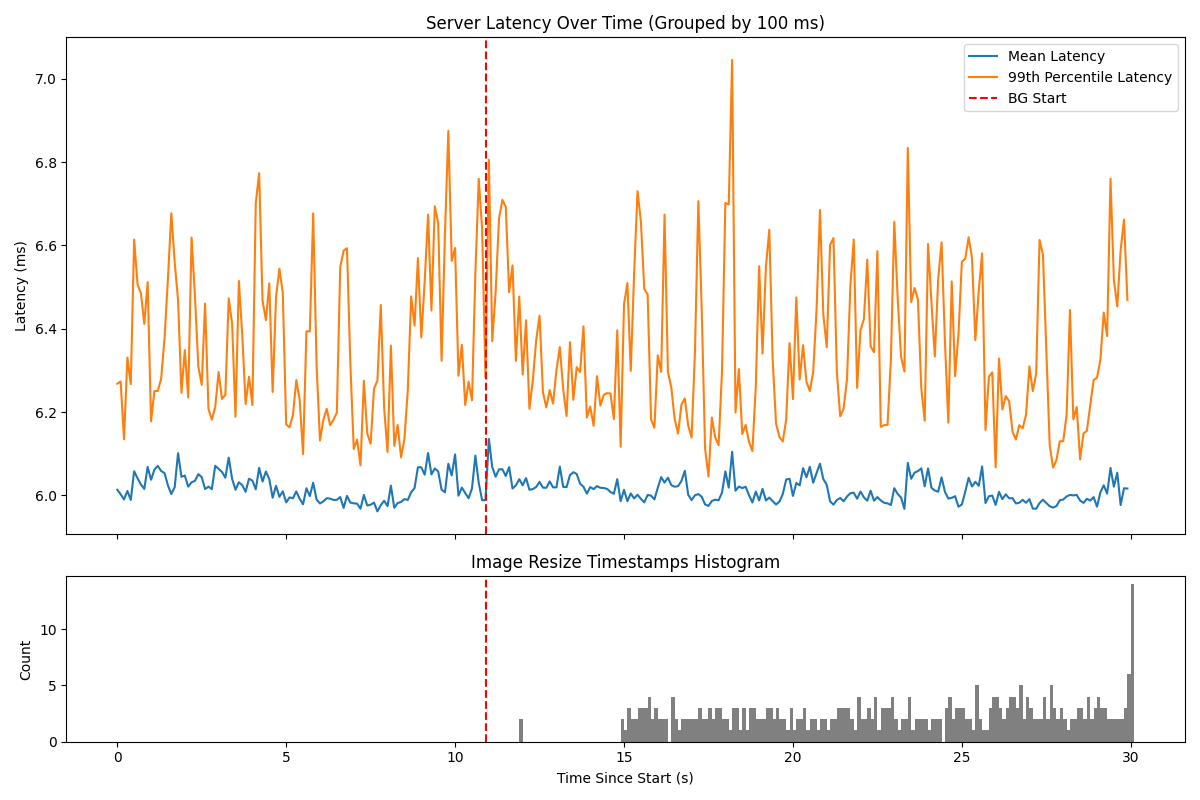
\includegraphics[width=\columnwidth]{graphs/unedited-rt-high-two.png}
        \caption{High load}\label{fig:unedited-rt-high-two}
    \end{subfigure}
    \vspace{4pt}
    \caption{Results of the same experiment, with LC running as a real time process}\label{fig:unedited-rt}
\end{figure}

We run the same experiment as in \autoref{s:intro}, but put the LC task in the
Fifo scheduling class, and leave BE tasks with the default process weight.
\autoref{fig:unedited-rt} shows the resulting measured latencies in the same low
and high load setting as previously. As expected, we see that Linux is able to
isolate the two very well. However, this is an untenable final solution because
of Fifo's run-to-completion scheduling, which is known to have a failure mode of
head-of-line (HoL) blocking, where long-running requests monopolize the CPU
while short requests wait in the queue. The Fifo scheduler also enforces not
only cross-core isolation between different priorities, but also a global
ordering within the same priority.

The takeaway is that Linux's current mechanism of scheduling classes can isolate
workloads effectively, but existing scheduling classes use scheduling
algorithms that are not a good fit for modern workloads.



